\chapter{État de l'art}

Intro

\section{PapARt}
Comme décrit dans l'introduction~\ref{chap:intro} Paper Augmented Reality Toolkit se présente sous la forme d'un kit de developpement permettant de créer des applications interactives en réalité augmentée de création de dessins ou de peinture (fig~\ref{fig:papartdemo}). L'idée est de proposé une technique numérique non intrusive pour faciliter une tâche complexe tel que le dessin tout en permettant à l'utilisateur de s'exprimer. % Parler de la conservation des proportions

\begin{figure}[H]
\centering
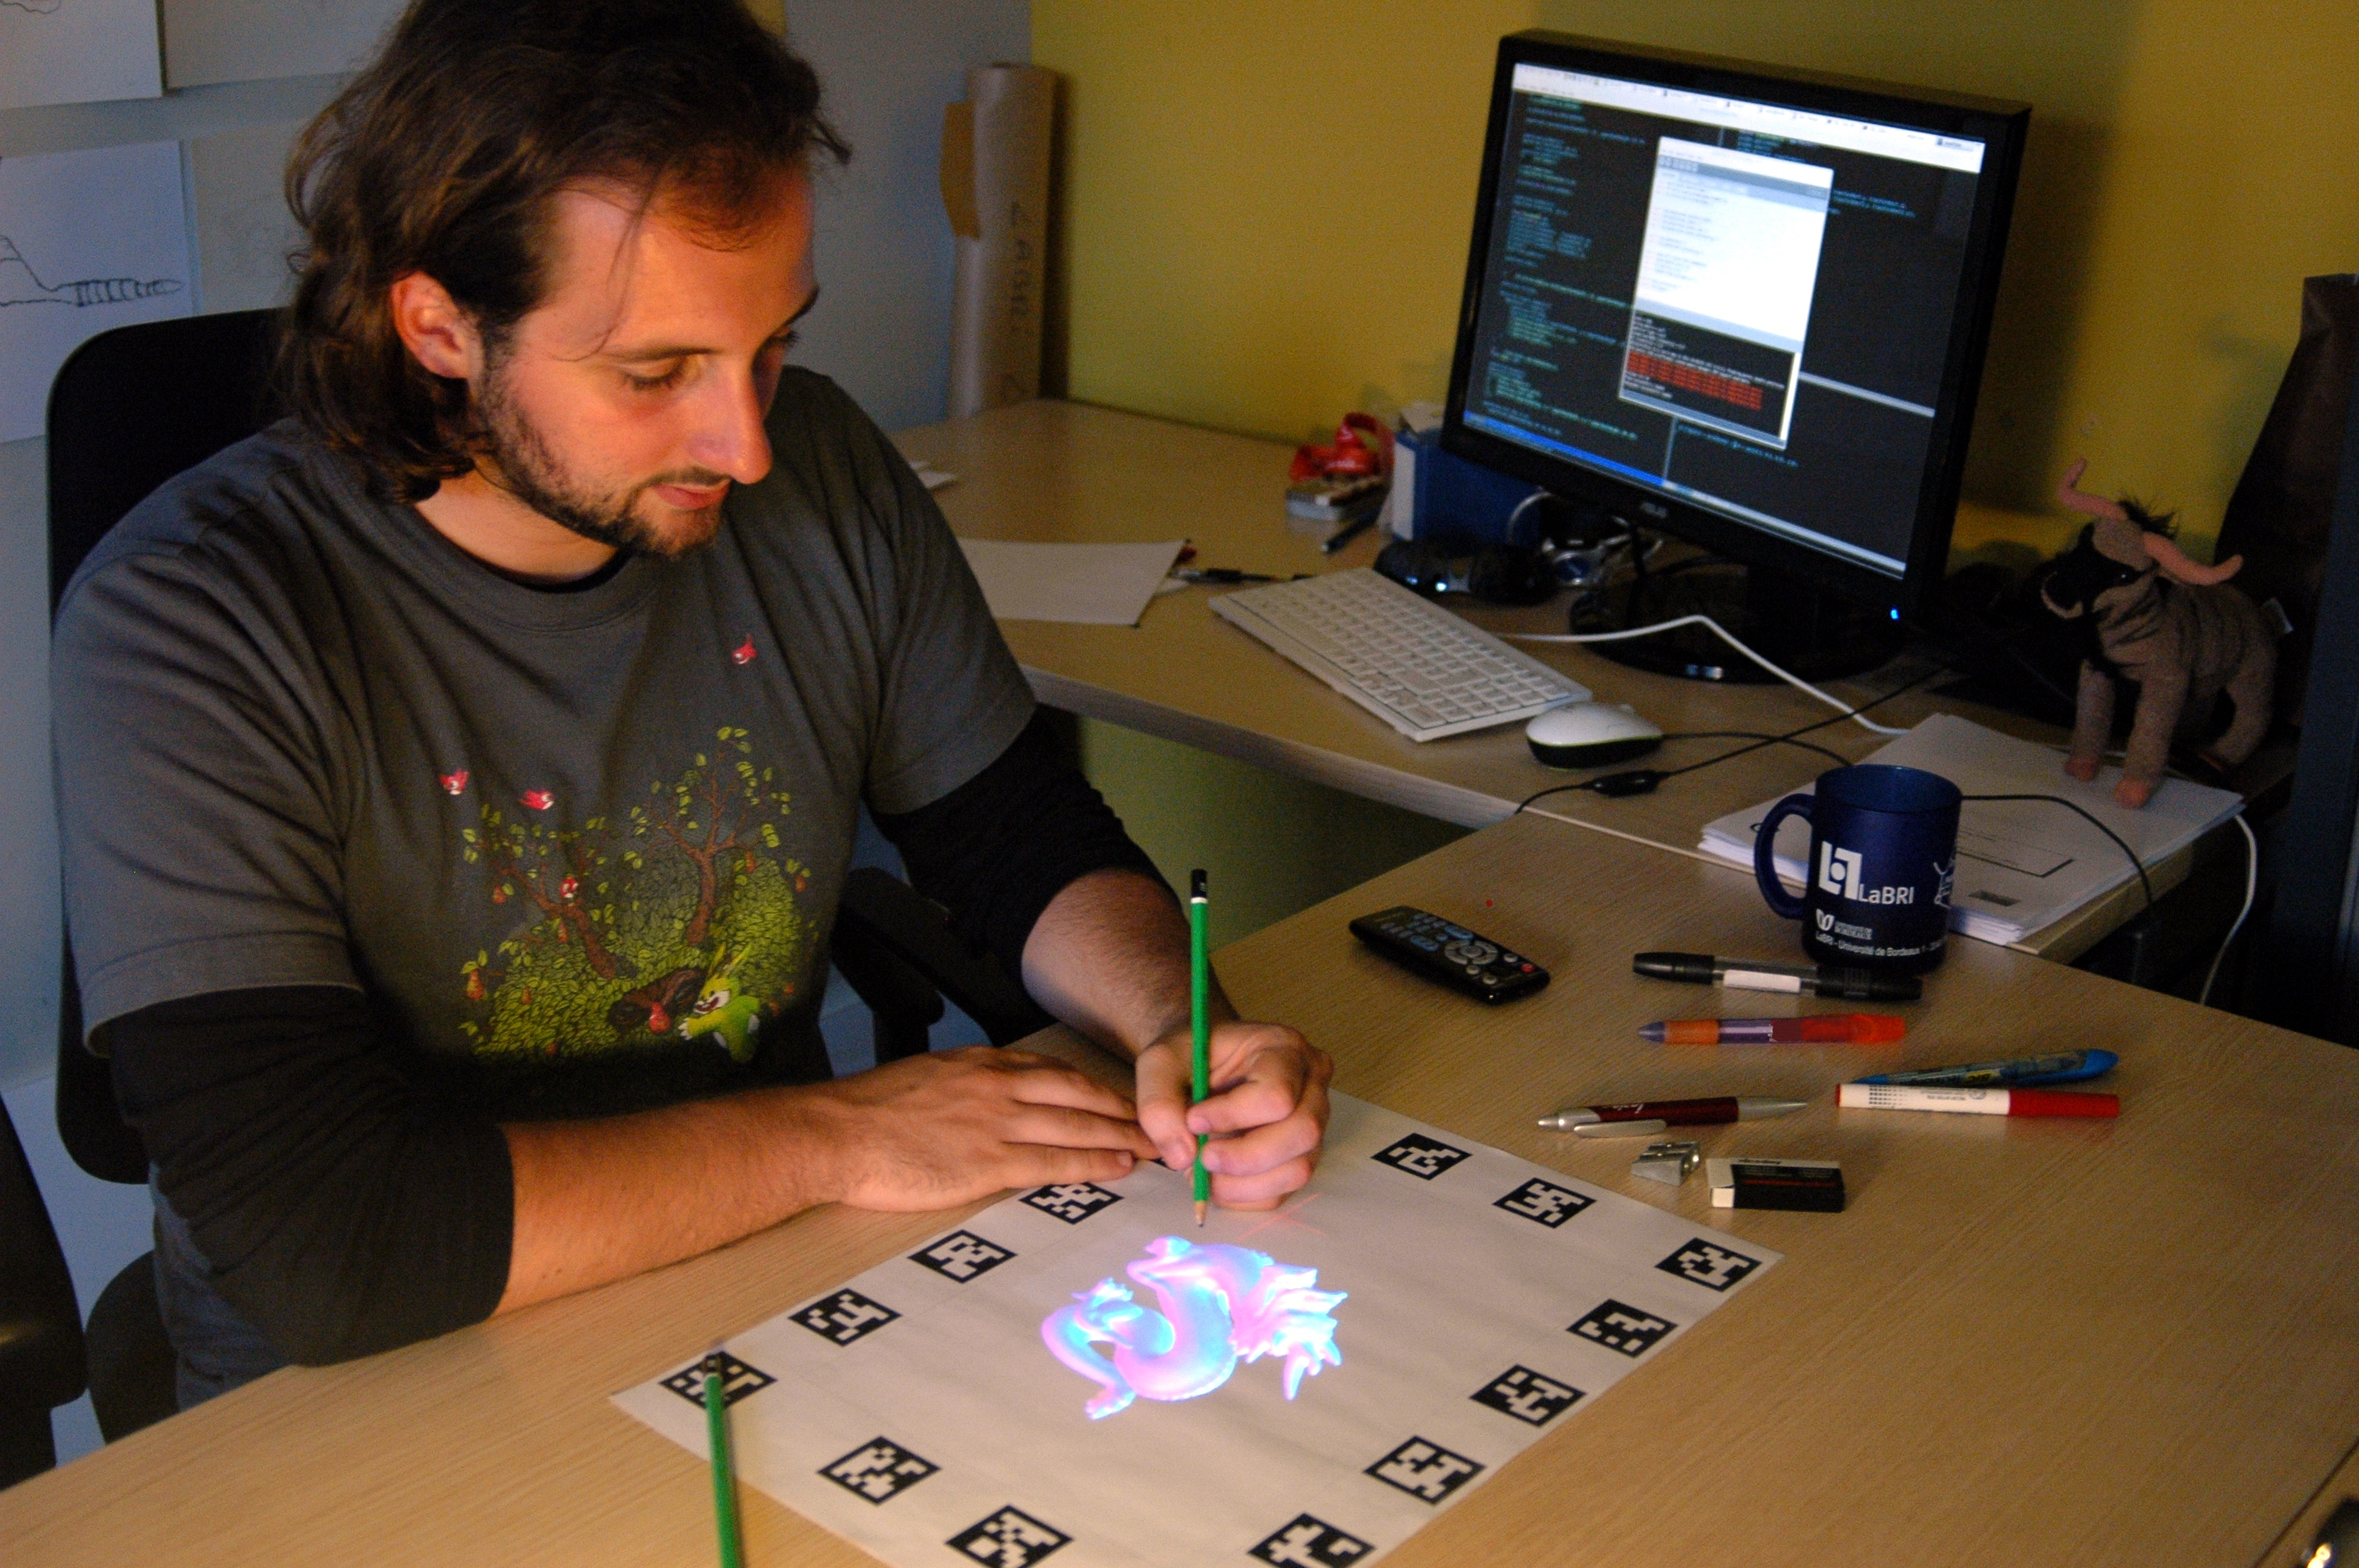
\includegraphics[width=0.65\textwidth]{images/papart-demo}
\caption{Démonstration PapARt\protect\footnotemark}
\label{fig:papartdemo}
\end{figure}
\footnotetext{Source: \href{https://team.inria.fr/potioc/fr/scientific-subjects_old/papart/}{Inria - PapARt}}

Le système interactif (fig~\ref{fig:papartsystem}) permettant d'utiliser tout le potentiel de PapARt est très spécifique. 

Il est composé de 2 dispositifs d'acquisitions, une caméra couleur observant la zone de travail pour venir y détecter les feuilles de papier qui serviront de base à la projection. Les feuilles de papier détectées par PapARt sont ornés de marqueurs ARToolKitPlus\footnote{\href{https://github.com/paroj/artoolkitplus}{https://github.com/paroj/artoolkitplus}} qui est une bibliothèque de détection de marqueurs fiduciaires \footnote{Expliquer}. Ces marqueurs une fois détectés permettent d'estimer assez précisément la position et le contenu de la feuille. PapARt se charge ensuite d'interpréter les marqueurs pour y projeter le contenu adéquat comme par exemple un dessin ou un menu.

Le deuxième dispositif d'acquisition est une caméra de profondeur qui a pour rôle de détecter les différents utilisateurs et les potentiels interactions grâce aux informations de profondeur. Les interactions peuvent être détecté soit sur le plan de la zone de travail, ce sont des interactions qualifiées de "touch" ou dans l'espace au dessus de la zone de travail, qu'on qualifiera de "pointage 3D".
Couplé a ces deux caméra, un projecteur est présent pour venir projeter dans les zones adéquates (i.e détectées via des feuilles de marqueur) le contenu numérique désiré. Pour avoir une représentation a l'échelle comme mentionné, il est nécessaire d'avoir un calibration caméras/projecteur très précise. Cette calibration très précise permet aux système complet d'avoir des capacités d'interaction et de manipulation (toucher, balayage, balayage a deux doigts) d'une tablette tactile.

\begin{figure}[H]
\centering
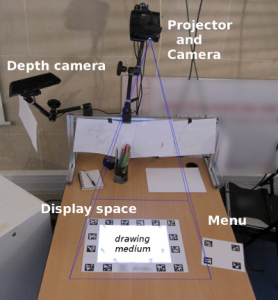
\includegraphics[width=0.4\textwidth]{images/papart-system}
\caption{Système interactif utilisant PapARt\protect\footnotemark}
\label{fig:papartsystem}
\end{figure}

\footnotetext{Source: \href{https://team.inria.fr/potioc/fr/scientific-subjects_old/papart/}{Inria - PapARt}}

Au delà des applications d'aide au dessins qui sont extrêmement nombreuses, PapARt ouvre un champ des possible assez large. Le rôle de RealityTech est d'explorer ce champ des possibles en améliorant PapARt et en fournissant de nouveau cas d'utilisation toujours plus innovants.



\section{Système de réalité augmentée spatiale}

\section{Bilan}